

\section{Experiment}




\subsection{Datasets}

\textbf{Brain cancer classification:}Dataset for detecting brain cancer is downloaded from Kaggle. It contains brain MRI images categorized into four classes: Three types of brain tumor,  and one healthy no Tumor class. 
% For tumor type classification task, 2870 images for training and 394 images for the test. 
For Meningioma and Glioma detection, 1437 and 1426 samples were used, respectively,  and they were split as train/ test data. Transforms rotation, Flipping, and normalizing.  Images were resized to 100$\times$100. 
\\
\textbf{Histopathologic cancer detection:} 
The samples are metastasic tissue images of lymph node cancer. Images are in size ,96 $\times$ 96, and the task is to classify the tissue samples. Each positive sample has a metastasic region, which is located in $32\times32$ neighborhood of each image sample. 
% Tumor tissue in the outer region of the patch does not influence the label. 
They were categorized into cancer and non-cancer classes. 2150 samples were chosen and randomly assigned to clients, and each split 62\% for train and 38\% for the test. We used horizontal Flipping, and images were normalized.

% \\\hl{A ro tu line 21 algorithm taarif kon va dorost kon notionesh ro}
\subsection{Network architectures}

\textbf{Deep learning models:}
The deep learning model used is a Convolutional Neural Network (CNN) with six layers of convolution stacked to 5 fully connected layers. The activation function used is ReLU. And dropout parameter (0.25). The last layer depends on the number of classes (4 or 2). Models are all trained and converged before implementing adversarial attacks.
They are trained with Cross-Entropy loss and with an SGD optimizer. Four models are trained separately. Two binary classification models are trained to detect Meningioma and Glioma from the healthy No Tumor class. One model is trained to detect cancer in HistoPathology images.

\textbf{Federated setting:}
Three clients are defined for the FL setup. The data is assigned randomly, and the clients have non-IID data distribution.
The FedAVG method is used to aggregate the models. The aggregation is weighed based on the length of the training dataset. Each client is trained for 20 epochs at the communication round. The total FL rounds are 50.

\subsection{Attack setting}

Each client is assigned 100 test samples to perform the adversarial attack. Each client is selected as the adversary, and the results are averaged at the end. 
% The attacks are conducted with different $\epsilon$ and gradient steps $\alpha$ to evaluate the effect on the final result. 
We use three metrics,
Clean accuracy is defined as the performance of models on uncorrupted test images, \textit{Attack Success Rate (ASR)}; how much an adversary can change the predicted labels produced by each model, \textit{Average Error Transferability Rate (AETR)} to evaluate transferability. An adversary might propose an attack by only selecting the samples that successfully fooled its own model. AETR measures how successfully these samples changed the target models' correct predictions. So unlike ASR, this metric doesn't count the examples that were initially misclassified by the victim model.\cite{papernot2017practical},

\begin{figure*}[h!]
     \centering
     \begin{subfigure}
         \centering
         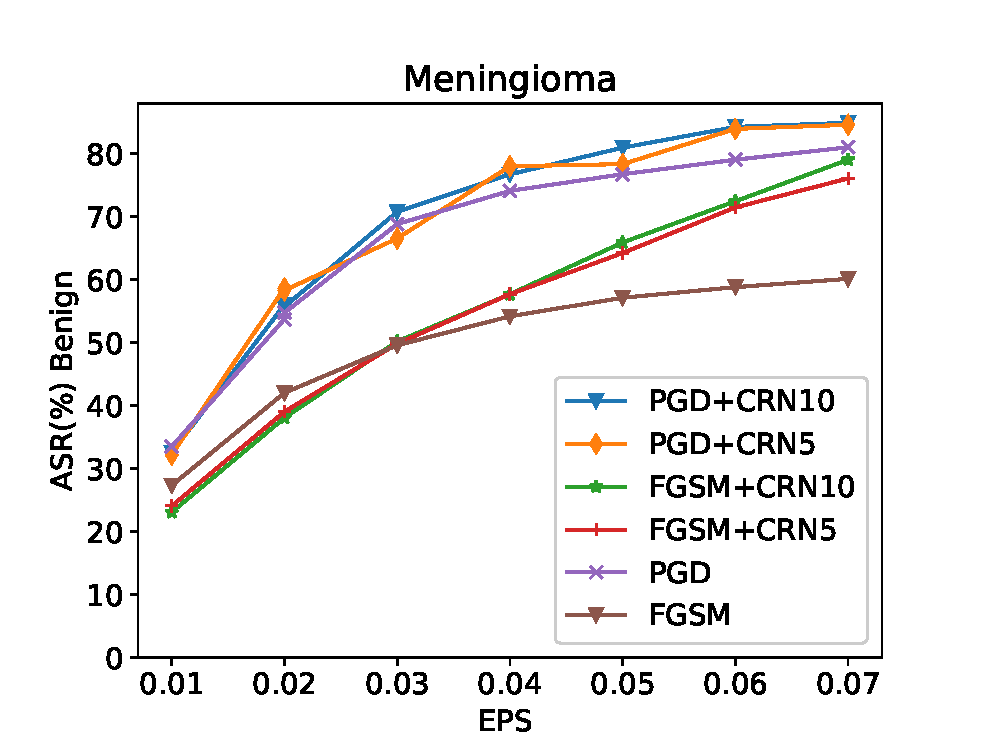
\includegraphics[width=0.32\textwidth]{Meningioma_ASR_EPS.eps}
          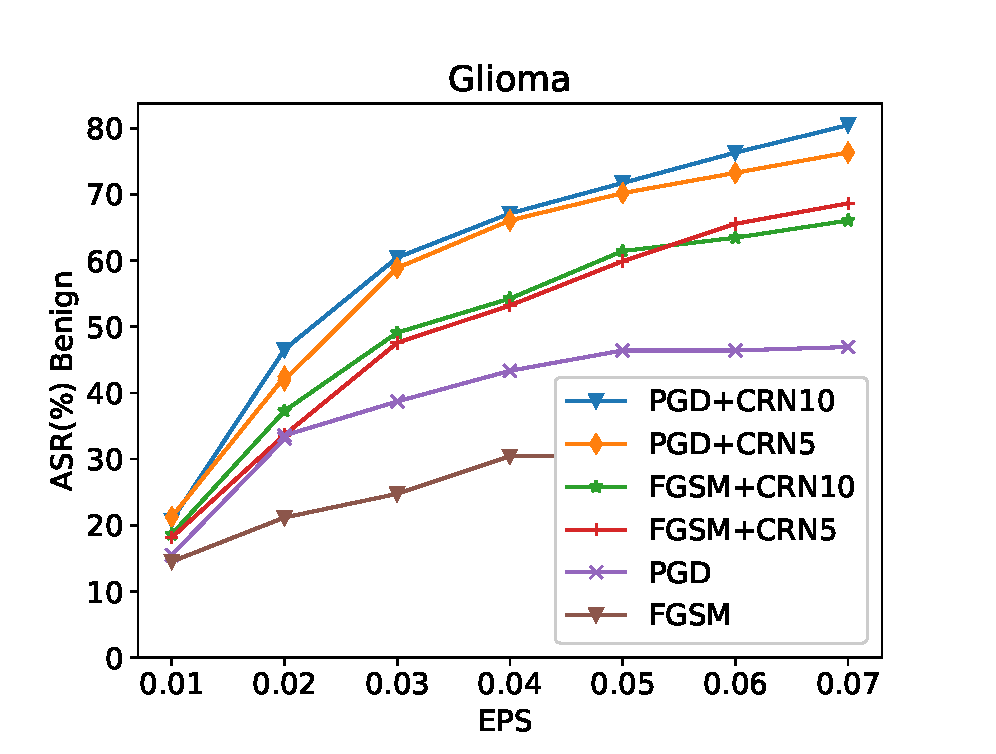
\includegraphics[width=0.32\textwidth]{Glioma_ASR_EPS.eps}
           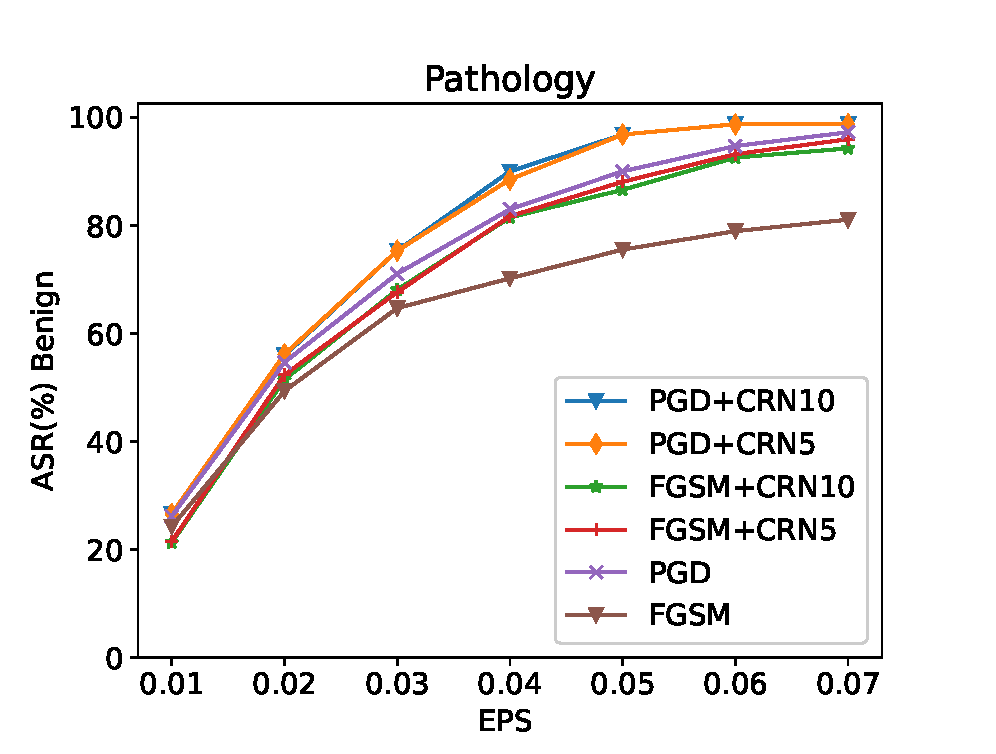
\includegraphics[width=0.32\textwidth]{Pathology_ASR_EPS.eps}
         \caption{Effect of $\epsilon$ on Average ASR on benign clients }
         \label{fig:AASR benign-EPS}
     \end{subfigure}
     \hfill
     \begin{subfigure}
          \centering
         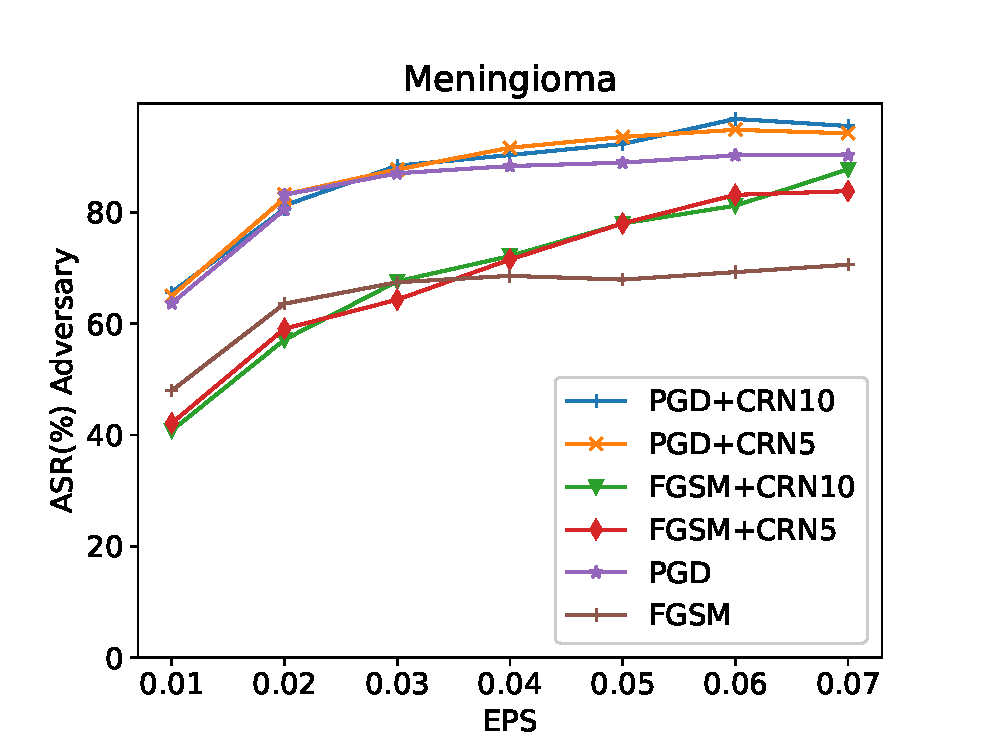
\includegraphics[width=0.32\textwidth]{Meningioma_others_EPS.eps}
          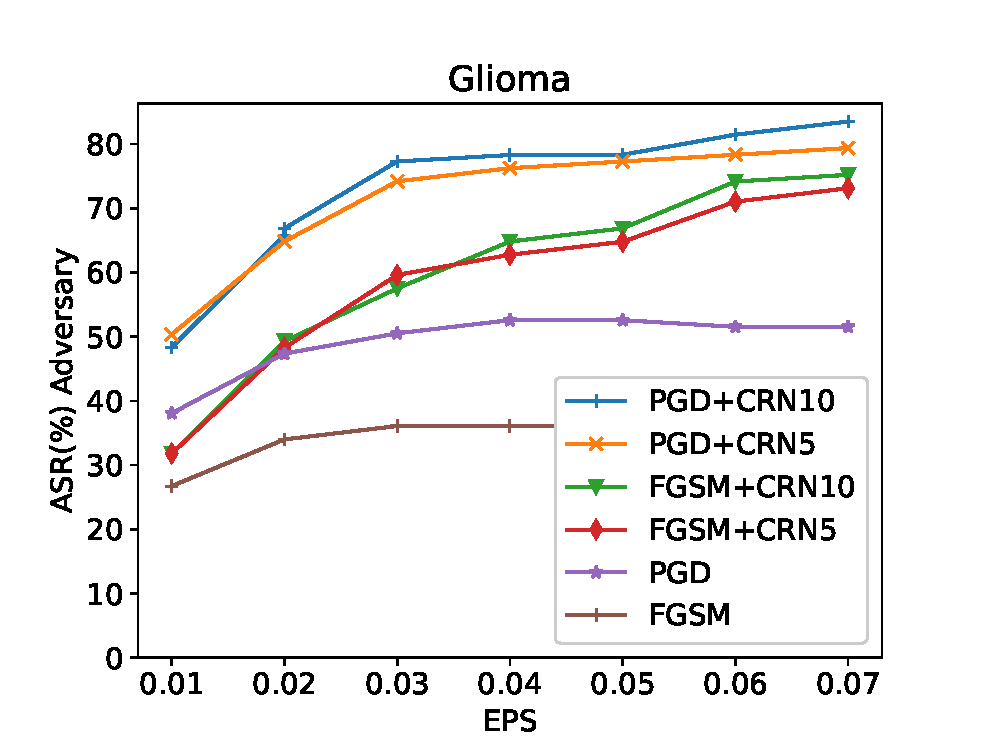
\includegraphics[width=0.32\textwidth]{Glioma_others_EPS.eps}
           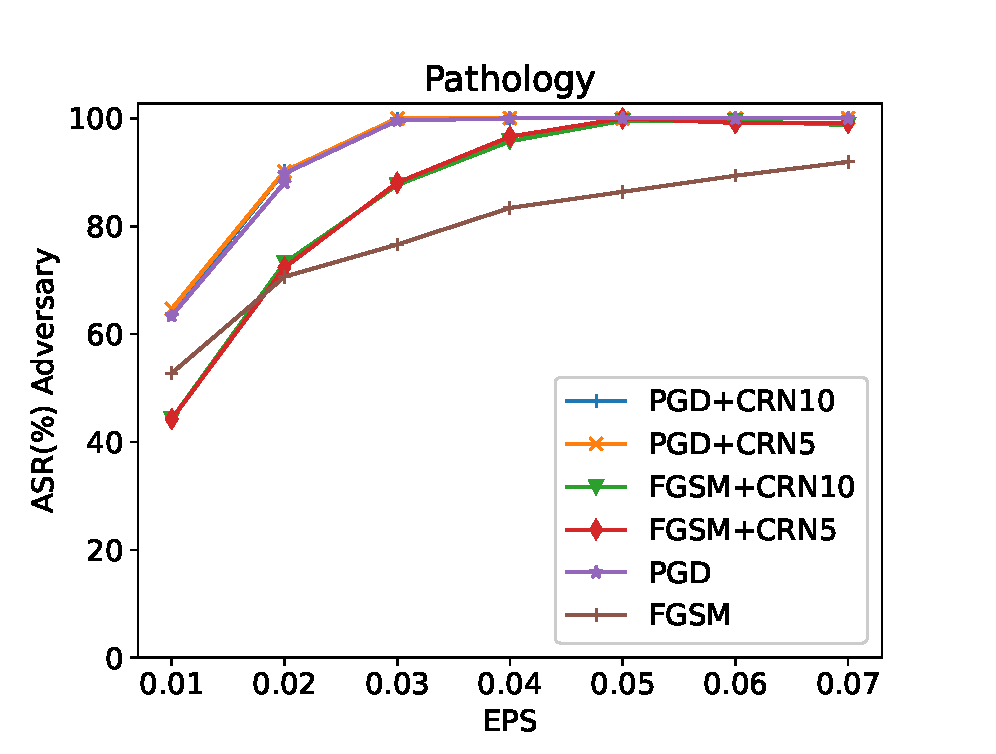
\includegraphics[width=0.32\textwidth]{Pathology_others_EPS.eps}
         \caption{Effect of $\epsilon$ on ASR on the advesarial client }
         \label{fig:AASR malignant-EPS}
     \end{subfigure}
     \hfill
        \caption{Effect of Error perturbation degree $\epsilon$ on attack transferability. FGSM and PGD attack with and without CRN initialization where performed. CRN initalizations used 10 models and another one loading 5.  ASR is calculated on benign and adversary clients. The results of with varying perturbation degrees. The higher ASR on benign clients shows higher transferability}
        \label{fig: epsilon graphs}
\end{figure*}

  Here, we expand the previous findings to the FL settings and discuss whether change in $\epsilon$ can lead to transferability. 
  
We perform three analysis to find important factors in attack success:
\begin{itemize}
    \item We investigate dependency of attacker on $\epsilon$. By visual inspection and ASR evaluation, and as a comparison to previously found optimal known values in centralized  setting.
    \item  We compare  efficiency of models, by discussing their attack preparation time and their ASR.
    \item We also see how attack step $\alpha$ can determine ASR.
\end{itemize}

